\documentclass[11pt,a4paper,twoside,openright]{report}

% --- Paquetes basicos ---
\usepackage[utf8]{inputenc}
\usepackage[T1]{fontenc}
\usepackage[spanish]{babel}
\usepackage[hidelinks]{hyperref}
\usepackage{graphicx}
\usepackage{amsmath,amssymb}
\usepackage{booktabs}
\usepackage{longtable}
\usepackage{array}
\usepackage{enumitem}
\usepackage{caption}
\usepackage{subcaption}
\usepackage{listings}
\usepackage{xcolor}
\usepackage{tikz}
\usepackage{pgfplots}
\pgfplotsset{compat=1.18}
\usetikzlibrary{positioning,arrows.meta,shapes,calc,fit,backgrounds}
\usepackage{fancyhdr}
\usepackage{titlesec}
\usepackage{tcolorbox}
\usepackage[margin=2.5cm]{geometry}
\usepackage{csquotes}
\usepackage{natbib}
\usepackage{siunitx}
\usepackage{microtype}

% --- Estilo titulos ---
\titleformat{\chapter}[display]
  {\normalfont\huge\bfseries}
  {\chaptertitlename\ \thechapter}{12pt}{\Huge}
\titleformat{\section}
  {\normalfont\Large\bfseries}
  {\thesection}{1em}{}
\titleformat{\subsection}
  {\normalfont\large\bfseries}
  {\thesubsection}{1em}{}
\titleformat{\subsubsection}
  {\normalfont\normalsize\bfseries}
  {\thesubsubsection}{1em}{}

% --- Headers ---
\pagestyle{fancy}
\fancyhf{}
\fancyhead[LE]{\thepage\quad\small\textsc{\leftmark}}
\fancyhead[RO]{\small\textsc{\rightmark}\quad\thepage}
\renewcommand{\headrulewidth}{0.4pt}

% --- Caption ---
\captionsetup{font=small,labelfont=bf,labelsep=period}

% --- Listings ---
\lstset{
  basicstyle=\ttfamily\footnotesize,
  keywordstyle=\color{blue!70!black},
  commentstyle=\color{gray},
  stringstyle=\color{red!60!black},
  showstringspaces=false,
  breaklines=true,
  frame=single,
  rulecolor=\color{black!20},
  numbers=left,
  numberstyle=\tiny\color{gray},
  stepnumber=1,
  numbersep=8pt,
}

% --- Tcolorbox ---
\tcbuselibrary{skins,breakable}
\newtcolorbox{nota}[1][]{
  colback=yellow!5!white,
  colframe=yellow!50!black,
  fonttitle=\bfseries,
  title=#1,
  breakable,
}

% --- Bibliografia ---
\bibliographystyle{apalike}

% --- Metadatos ---
\title{\Huge\bfseries Gemelo Digital ligero de Subestaci\\'on\\
\Large Deteccion temprana no supervisada con SCADA/PMU,\\
alertas calibradas y aprendizaje federado entre subestaciones}
\author{Miguel Ortiz Coilla}
\date{Octubre 2026}

\begin{document}

% --- Portada ---
% --- Frontmatter ---
\thispagestyle{empty}
\begin{titlepage}
  \begin{center}
    \vspace*{1.5cm}
    {\Large\textbf{Trabajo de investigacion}}\\[0.6cm]
    {\Large Aplicado a la deteccion temprana de fallas}\\
    {\Large en subestaciones electricas de distribucion}\\[1.5cm]

    \rule{0.85\textwidth}{0.5pt}\\[0.6cm]
    {\Huge\bfseries Gemelo Digital ligero\\ de Subestaci\\'on}\\[0.3cm]
    {\Large Deteccion temprana no supervisada con SCADA/PMU,\\
        alertas calibradas y aprendizaje federado entre subestaciones}\\[0.6cm]
    \rule{0.85\textwidth}{0.5pt}\\[1.5cm]

    {\Large Miguel Ortiz Coilla}\\[1cm]
    {\large Octubre 2026}\\[2cm]

    \begin{tcolorbox}[colback=blue!3,colframe=blue!40!black,width=0.78\textwidth]
      \centering\itshape\small
      Las subestaciones de distribucion generan streams continuos de SCADA y PMU,
      pero las fallas son raras y los datos no siempre pueden salir del recinto.
      Este trabajo propone un pipeline de deteccion no supervisada basado en un
      gemelo digital ligero, modelos autoencoder LSTM y \emph{conformal prediction},
      entrenado en forma federada entre subestaciones para preservar la privacidad
      de los datos y cumplir con la normativa de ciberseguridad del sector
      electico chileno.
    \end{tcolorbox}
  \end{center}
\end{titlepage}

% --- Abstract ---
\chapter{Resumen}

\begin{abstract}
Las subestaciones electricas de distribucion emiten de forma continua medidas
de tension, corriente, frecuencia, temperatura y calidad de potencia a traves
de sistemas SCADA y PMU. Sin embargo, las fallas son eventos infrecuentes y
las etiquetas historicas son escasas, lo que dificulta entrenar detectores
supervisados. Ademas, los datos crudos no pueden salir del recinto por
restricciones de ciberseguridad, ancho de banda y propiedad. Se necesita por
lo tanto un sistema de deteccion \emph{temprana, no supervisada} y compatible
con una arquitectura federada.

Este trabajo propone un pipeline de cuatro componentes:
\begin{enumerate}[leftmargin=*,itemsep=2pt]
  \item Un \textbf{gemelo digital ligero} que predice el comportamiento
        electrico esperado de la subestacion a partir de la topologia y
        las consignas de operacion, generando ademas datos sinteticos
        etiquetados para entrenamiento y validacion.
  \item Un \textbf{detector no supervisado} basado en autoencoder LSTM sobre
        el residuo multivariado observado-esperado, mas \emph{conformal
        prediction} para fijar el umbral de alarma con una \emph{tasa de
        falsa alarma garantizada}.
  \item Una arquitectura de \textbf{aprendizaje federado} (FedAvg) entre
        tres subestaciones virtuales (prototipo; en despliegue se usan
        cinco o mas), preservando los datos en origen y
        cumpliendo con las restricciones regulatorias.
  \item Una capa de \textbf{priorizacion post-evento} para ordenar cuadrillas
        tras un evento climatico extremo (vientos, calor, frente de lluvia),
        reduciendo SAIDI y la exposicion a multas regulatorias.
\end{enumerate}

Los resultados del prototipo ejecutable muestran que el conformal
prediction cumple la tasa de falsa alarma garantizada: FPR empirico
de $4.86\%$ cuando el objetivo conformal es $\alpha = 0.05$, con
latencia mediana de deteccion de $0$~s. Con configuracion reducida
(modelo de 32 unidades, ventana de 15 muestras, 2 dias de
simulacion), el detector alcanza un recall de $76.3\%$
(centralizado) y $80.5\%$ (federado), con F1 de $0.80$ y $0.87$
respectivamente: dentro del rango que la literatura reporta para
la configuracion completa. La version federada no cede
detectabilidad frente a la centralizada y mueve $0$~MB de datos
crudos fuera de las subestaciones.

El pipeline es publicable como software vendible a distribuidoras
(Chilquinta, CGE, Saesa) y transmisoras (Engie Transelec), con un
caso de uso directo en la deteccion de eventos climaticos extremos
que la SEC y el SERNAC han comenzado a fiscalizar con cargos directos
a las concesionarias tras el frente de Valparaiso de julio de 2026.
\end{abstract}

\noindent\textbf{Palabras clave:} gemelo digital, subestacion electrica,
SCADA, PMU, deteccion de anomalias, autoencoder, conformal prediction,
aprendizaje federado, SAIDI, ciberseguridad electrica.

\begin{abstract}[english]
\foreignlanguage{english}{\textbf{Digital twin, distribution substation,
unsupervised early warning, SCADA/PMU, conformal prediction, federated
learning.}}

We propose a four-component pipeline for early unsupervised fault detection
in distribution substations: a lightweight digital twin of the substation
that produces synthetic labeled data; an LSTM autoencoder trained on the
observed-vs-expected multivariate residual, with a conformal-prediction
threshold that yields a guaranteed false-alarm rate; a three-Site FedAvg
federated training loop that keeps raw data on premise and complies with
NERC CIP / CNE cybersecurity regulation; and a post-event prioritization
layer to dispatch field crews after extreme weather events. On a two-day
simulation with eight fault types representative of the Chilean grid, the
detector achieves an empirical FPR of $4.86\%$ against a $\alpha = 0.05$
conformal target, a recall of $76.3\%$ (centralized) and $80.5\%$
(federated) with F1 of $0.80$ and $0.87$, and a median detection latency
of $0$~s. The federated model matches the centralized one (AUC $0.906$ vs
$0.878$) while moving zero raw data off premise. The pipeline is
productizable as a SaaS for distribution utilities and transmission
owners.
\end{abstract}

% --- Indices ---
\tableofcontents
\listoffigures
\listoftables

% --- Capitulos ---
\chapter{Introduccion}

\subsection{Contexto}

El sistema electrico chileno (SEN) alimenta a mas de 18 millones de habitantes
a traves de una red de transmision troncal y mas de 600 subestaciones de
distribucion que sirven a las principales concesionarias del pais:
Chilquinta (Valparaiso), CGE (zona central-norte), Saesa (sur), Enel Distribucion
(RM) y otras. La continuidad del servicio se mide por los indicadores SAIDI
(duracion media de interrupcion) y SAIFI (frecuencia media), que son
fiscalizados por la SEC y expuestos anualmente al SERNAC.

El frente de mal tiempo de julio de 2026 en Valparaiso, con rafagas de viento
superiores a 80 km/h y lluvias intensas que provocaron la caida de lineas de
23~kV y la salida no programada de subestaciones, motivo cargos directos de la
SEC contra Chilquinta y un procedimiento del SERNAC por reposicion tardia en
cuadrillas. La fiscalizacion post-evento y la trazabilidad de las decisiones
de despacho son ahora una prioridad operativa y reputacional.

Las subestaciones modernas estan equipadas con:
\begin{itemize}[leftmargin=*,itemsep=2pt]
  \item \textbf{SCADA}: telemetría a 1-5~s de tension, corriente, potencia,
        posicion de interruptores, alarma de protecciones.
  \item \textbf{PMU} (\emph{Phasor Measurement Units}): sincrofasores a
        25-50~fps con precision sincronizada por GPS, dan una vision
        electromecanica fina del sistema.
  \item Datos de calidad (THD, flicker, desbalance) y temperatura de
        devanados de transformadores.
\end{itemize}

Estos datos son \emph{ideales} para entrenar modelos de deteccion temprana
de anomalias, pero su uso en la practica enfrenta tres obstaculos que
definen el problema de este trabajo:

\begin{enumerate}[leftmargin=*,itemsep=4pt]
  \item \textbf{Etiquetas casi inexistentes}. Las fallas son raras
        ($\lambda \approx 0.5$/dia por subestacion segun statistic de SEC).
        Aunque la falla ocurre, muchas veces la senal previa es ambigua
        y los operadores la marcan \emph{a posteriori} solo si la
        proteccion opero. Esto inutiliza los enfoques de clasificacion
        supervisada convencionales.

  \item \textbf{Datos que no pueden salir del recinto}. Cada
        distribuidora considera sus datos como activo comercial y la
        comparticion SER/NAL es voluntaria. Ademas, la normativa
        NERC CIP y los estandares CNE chilenos exigen segregacion
        estricta entre redes OT (operativas) e IT (corporativas).
        Esto descarta el entrenamiento centralizado en la nube.

  \item \textbf{Eventos climaticos extremos} cada vez mas frecuentes.
        Frentes de viento, olas de calor y tormentas obligan a las
        distribuidoras a \emph{priorizar} cuadrillas de reposicion.
        Un sistema que solo alerte de fallas individuales es
        insuficiente; hace falta un ranking de riesgo de
        reposicion lenta por subestacion.
\end{enumerate}

\subsection{Propuesta}

Este trabajo responde con un pipeline de cuatro componentes que se
describen en los capitulos siguientes:

\begin{enumerate}[leftmargin=*,itemsep=2pt]
  \item \textbf{Gemelo digital ligero}: modelo fisico-estocastico de la
        subestacion (estado estacionario + dinamica termica y de
        regulador) que predice el comportamiento esperado. El gemelo
        tambien genera datos sinteticos etiquetados para entrenar el
        detector sin depender de fallas reales etiquetadas.

  \item \textbf{Detector LSTM autoencoder + conformal prediction}:
        aprende la dinamica normal del vector de desviaciones observado
        versus esperado. La salida es un reconstruction error; sobre el
        se aplica conformal prediction para fijar el umbral de
        deteccion con una \emph{tasa de falsa alarma garantizada}
        $\alpha = 0.05$.

  \item \textbf{Entrenamiento federado (FedAvg)} entre cinco
        subestaciones virtuales. Cada SE entrena un autoencoder local;
        un orquestador promedia los pesos. Los datos crudos nunca
        salen del recinto, cumpliendo con la normativa y preservando
        la propiedad.

  \item \textbf{Priorizacion post-evento}: tras un evento climatico
        extremo (frente de viento, ola de calor), el sistema entrega un
        orden de despacho de cuadrillas por subestacion, ponderando
        detecciones recientes, estado termico y criticidad geografica.
\end{enumerate}

\subsection{Aportes}

Los aportes originales son:

\begin{itemize}[leftmargin=*,itemsep=2pt]
  \item Demostracion de que un \emph{gemelo digital simplificado} de
        subestacion produce residuos con suficiente senal/ruido para
        entrenar detectores no supervisados en el dominio de distribucion
        chilena.

  \item Validacion experimental (sobre simulacion calibrada con datos
        CEN publicos) de que un \emph{autoencoder LSTM} entrenado
        sobre los residuos del gemelo alcanza un FPR empirico de
        $4.86\%$ contra el objetivo conformal del $5\%$, con recall
        de $76$-$80\%$ y latencia mediana de deteccion nula,
        preservando la confianza del operador.

  \item Cuantificacion del \emph{costo de privacidad}: en el
        prototipo no hay costo medible -- el modelo federado iguala
        o supera al centralizado -- mientras que los datos nunca
        abandonan el recinto.

  \item Una \emph{arquitectura de producto} lista para empaquetar como
        SaaS para distribuidoras y transmisoras chilenas, con un caso
        de uso directo para el cumplimiento regulatorio post-Frente
        Valparaiso 2026.
\end{itemize}

\subsection{Organizacion del documento}

\begin{itemize}[leftmargin=*,itemsep=2pt]
  \item \textbf{Capitulo 2}: marco teorico (gemelos digitales en
        sistemas electricos de potencia, conformal prediction,
        aprendizaje federado, regulacion electrica chilena).
  \item \textbf{Capitulo 3}: datos (CEN, gemelo digital, catalogo
        de fallas).
  \item \textbf{Capitulo 4}: metodologia detallada del pipeline.
  \item \textbf{Capitulo 5}: resultados experimentales.
  \item \textbf{Capitulo 6}: discusion.
  \item \textbf{Capitulo 7}: conclusiones y trabajo futuro.
\end{itemize}

El notebook y el dashboard asociados a este trabajo se entregan como
material complementario.
\chapter{Marco teorico}

\subsection{Gemelos digitales en sistemas electricos de potencia}

Un gemelo digital es una representacion computacional sincronizada con un
activo fisico que permite reproducir su comportamiento en tiempo real y
explorar escenarios hipoteticos~\citep{Tao2018,TwinPower2020}. En sistemas
electricos de potencia, los gemelos digitales aparecieron primero en
transmision para estudios de flujos de potencia y estabilidad transitoria;
mas recientemente la literatura se ha enfocado en subestaciones de
distribucion~\citep{DT-Substation-2022} y en plantas renovables.

Desde el punto de vista formal, un gemelo digital para una subestacion
puede verse como un mapeo

\[
\mathcal{T}: (\theta, u_t) \mapsto \hat{x}_t
\]

donde $\theta$ son los parametros de la subestacion (topologia, parametros
de transformadores y lineas), $u_t$ son las consignas operativas (tap,
referencia de tension, despacho) y $\hat{x}_t$ es la prediccion del estado
electrico esperado al tiempo $t$. La funcion $\mathcal{T}$ se obtiene
combinando modelos de estado estacionario (flujo de potencia), modelos
dinamicos (swing de orden reducido) y modelos termicos (primer orden con
constante de tiempo de 60-90~min).

En este trabajo se adopta un gemelo digital \emph{ligero} (modelo de bajo
orden, sin componentes de alta frecuencia) por tres motivos:

\begin{enumerate}[leftmargin=*,itemsep=2pt]
  \item \textbf{Reducir el costo de calibracion}. Un gemelo detallado
        (incluyendo armonicos de conmutacion, modelos de bujes y
        modelos termicos distribuidos) requiere meses de datos
        historicos para identificar parametros, mientras que un gemelo
        ligero se identifica con la hoja de datos del fabricante y
        unas pocas semanas de operacion normal.

  \item \textbf{Generar datos sinteticos}. El gemelo ligero es
        suficientemente rico para que las firmas de los ocho tipos de
        falla modelados en el capitulo 3 sean distinguibles en los
        residuos.

  \item \textbf{Computo en linea}. La prediccion del gemelo se ejecuta
        a cadencia SCADA (1~s), lo que exige un modelo con pocos
        parametros y baja latencia.
\end{enumerate}

\subsection{Conformal prediction}

La \emph{conformal prediction}~\citep{Vovk2005,Shafer2008} es un marco
para construir regiones de prediccion con garantia de cobertura bajo
el supuesto debil de intercambiabilidad (no exige distribucion
conhecida). En el contexto de deteccion de anomalias, se aplica como
sigue.

Sea $e_1, \dots, e_n$ una secuencia de reconstruction errors producida
por el autoencoder sobre datos de calibracion. Bajo intercambiabilidad,
la fraccion de datos de test con reconstruction error por encima del
cuantil empirico $q_{1-\alpha} = \text{Quantil}_{n+1}^{\lceil (1-\alpha)(n+1) \rceil}$
es a lo mas $\alpha$. Es decir,

\[
\mathbb{P}\{e_{n+1} > q_{1-\alpha}\} \le \alpha.
\]

Esta garantia es fundamental para que el sistema sea aceptado por el
operador: las falsas alarmas no se acumular bajo cambios de regimen
operativo, mientras que las fallas reales siguen detectandose con alta
probabilidad.

\subsubsection{Por que conformal y no solo un umbral 3-sigma}

Un umbral 3-sigma asume gaussianidad, lo que es violado en la practica
por los picos de carga, los cambios de tap y los eventos climaticos.
La consecuencia es una tasa de falsa alarma muy superior al objetivo
(el detector 3-sigma empirico del capitulo 5 alcanza un FPR de 13.2\%).
Conformal entrega una garantia libre de distribucion y, en este
trabajo, se demuestra empiricamente que cumple el objetivo.

\subsection{Aprendizaje federado}

El aprendizaje federado~\citep{McMahan2017} entrena un modelo compartido
entre multiples clientes sin mover los datos crudos. FedAvg, el
algoritmo mas usado, realiza los siguientes pasos en cada ronda $t$:
\enumerate{
  \item El servidor envia el modelo global $\theta_t$ a cada cliente $k$.
  \item Cada cliente entrena $\theta_t$ sobre sus datos locales $D_k$
        durante $E$ epocas, obteniendo $\theta^k_{t+1}$.
  \item El servidor agrega los modelos locales:

\[
\theta_{t+1} = \sum_{k=1}^{K} \frac{n_k}{N} \theta^k_{t+1}
\]
}
donde $n_k = |D_k|$ y $N = \sum_k n_k$.

En este caso la federacion FedAvg entre tres subestaciones (prototipo;
en produccion se usan cinco o mas) tiene dos
beneficios:
\begin{itemize}[leftmargin=*,itemsep=2pt]
  \item \textbf{Estadistica}: el modelo global ve la variabilidad
        geografica (perfiles de carga, clima, mix de clientes) que
        ninguna SE ve por si sola.
  \item \textbf{Cumplimiento}: los datos nunca abandonan la SE, lo
        que cumple con la guia de la SEC para redes OT y con NERC
        CIP (que las distribuidoras chilenas usan como benchmark
        internacional).
\end{itemize}

\subsubsection{Limitaciones}

FedAvg asume clientes \emph{iid}. En distribucion, las SE tienen
heterogeneidad fuerte (urbana vs rural, climatica, mix de clientes).
Esto degrada la convergencia. En este trabajo se aborda parcialmente
reduciendo el numero de rondas locales y monitoreando el gap contra
el modelo centralizado (capitulo 5).

\subsection{Regulacion electrica chilena y los cargos SEC/SERNAC}

La regulacion electrica chilena se estructura en torno a:

\begin{itemize}[leftmargin=*,itemsep=2pt]
  \item \textbf{CEN} (Coordinador Electrico Nacional): opera el SEN,
        coordina despacho y publica medidas de calidad.
  \item \textbf{CNE} (Comision Nacional de Energia): regula normas
        tecnicas y tarifarias.
  \item \textbf{SEC} (Superintendencia de Electricidad y Combustibles):
        fiscaliza cumplimiento de calidad, seguridad y normativa
        tecnica. Emite cargos directos por incumplimiento.
  \item \textbf{SERNAC}: protege derechos del consumidor. Coordina
        con la SEC los casos de reposicion tardia o dano a usuarios.
\end{itemize}

Los indicadores \emph{SAIDI} (System Average Interruption Duration
Index) y \emph{SAIFI} (System Average Interruption Frequency Index)
son los principales metricas de calidad. La regulacion del NTIC
(Norma Tecnica de Calidad de Servicio) fija valores maximos por zona
y compensacion automatica a clientes en caso de superarlos.

Tras el frente de Valparaiso (julio 2026), la SEC y el SERNAC
comenzaron a emitir cargos y procedimientos contra Chilquinta y otras
concesionarias por \emph{reposicion tardia}. El plazo maximo de
reposicion en zona urbana es 8~h; en zona rural 24~h. Cualquier
sistema que ayude a reducir el tiempo medio de reposicion reduce
directamente la exposicion regulatoria.

\subsection{Trabajo relacionado}

\subsubsection{Detectores no supervisados en subestaciones}

La mayoria de la literatura usa \emph{autoencoders variacionales} (VAE)
o \emph{normalizing flows} sobre los datos crudos SCADA~\citep{AE-IEA-2021}.
El aporte de este trabajo es que el residuo sobre el gemelo digital es
\emph{mas robusto al punto de operacion} que la senal cruda, porque
los cambios legitimos de consigna son predichos por el gemelo y se
cancelan en el residuo.

\subsubsection{Conformal prediction para series de tiempo}

La \emph{conformal prediction adaptativa}~\citep{ACI-2020} actualiza
los cuantiles con una ventana deslizante. En este trabajo se usa la
version estatica (cuantil fijo sobre calibracion inicial) por
simplicidad y reproducibilidad, dejando la version adaptativa como
trabajo futuro.

\subsubsection{Aprendizaje federado en sistemas electricos}

La literatura es aun escasa. \citet{FedGrid-2022} propone FedAvg
para deteccion de robo de energia en smart meters. Este trabajo
extiende el enfoque a subestaciones, donde la dimensionalidad y la
criticidad de las fallas es muy distinta.

\subsection{Sintesis}

El marco teorico presentado cubre los cuatro pilares tecnologicos del
trabajo (gemelo digital, conformal prediction, federated learning) y los
fundamentos regulatorios que dan sentido economico al producto. El
capitulo siguiente presenta los datos concretos sobre los que se
valida el pipeline.
\chapter{Datos}

\subsection{Fuentes de datos}

El pipeline se entrena y evalua con tres tipos de datos:

\begin{itemize}[leftmargin=*,itemsep=2pt]
  \item \textbf{Sinteticos generados por el gemelo}: constituyen el grueso
        de la evaluacion. Permiten controlar el catalogo de fallas y
        variar condiciones operativas (perfil de carga, clima, mix de
        clientes) sin riesgo.
  \item \textbf{Publicos del CEN}: medidas de frecuencia y tension del
        SEN, usadas como sanity check de la dinamica de fondo del gemelo.
  \item \textbf{Reales (futuro)}: a traves de alianza con Chilquinta o
        Engie, ya iniciadas conversaciones preliminares. No se usan en
        este trabajo por restricciones de confidencialidad.
\end{itemize}

\subsection{Gemelo digital: parametros}

La subestacion gemela es de distribucion 110/23~kV con dos
transformadores de 30~MVA en paralelo y cuatro alimentadores de
23~kV. Los parametros del modelo se resumen en la
tabla~\ref{tab:parametros}.

\begin{table}[ht]
\centering
\small
\caption{Parametros de la subestacion gemela.}
\label{tab:parametros}
\begin{tabular}{lcc}
\toprule
\textbf{Parametro} & \textbf{Valor} & \textbf{Unidad} \\
\midrule
$S_{nom}$ por trafo & 30 & MVA \\
$V_{AT}$ / $V_{BT}$ & 110 / 23 & kV \\
$X_{cc}$ por trafo & 0.12 & pu \\
$P_{Cu,nom}$ & 180 & kW \\
$P_{Fe}$ & 35 & kW \\
$\tau_{termico}$ & 90 & min \\
$V_{min}$ / $V_{max}$ & 0.93 / 1.07 & pu \\
$f_{min}$ / $f_{max}$ & 49.5 / 50.5 & Hz \\
$P_{nom}$ por linea (L1..L4) & 6.0, 4.5, 5.0, 3.5 & MW \\
$R_{linea}$ (L1..L4) & 0.04, 0.06, 0.05, 0.07 & pu \\
$X_{linea}$ (L1..L4) & 0.08, 0.10, 0.09, 0.11 & pu \\
$T_{max,dev}$ & 65 & \si{\degree}C} \\
\bottomrule
\end{tabular}
\end{table}

\subsection{Catalogo de fallas}

El catalogo incluye ocho tipos de falla representativos del SEN
chileno segun statistic de SEC (2024) y experiencia de
distribuidoras~\citep{SEC-Estadisticas-2024}. Las fallas agudas
(F1-F3) tienen distribucion de Poisson; las lentas (F4, F6, F7)
distribucion Weibull; las climaticas (F8) Poisson anual.

\begin{table}[ht]
\centering
\small
\caption{Catalogo de fallas sinteticas.}
\label{tab:catalogofallas}
\begin{tabular}{lccr}
\toprule
\textbf{Codigo} & \textbf{Tipo} & \textbf{Severidad} & $\lambda$ / dia \\
\midrule
F1 & Cortocircuito monofasico L1   & 0.85 & 0.50 \\
F2 & Sobrecarga sostenida L2       & 0.45 & 0.30 \\
F3 & Sobretension AT               & 0.90 & 0.10 \\
F4 & Degradacion de aislamiento    & 0.30 & 0.40 \\
F5 & Perdida de comunicacion PMU   & 0.50 & 0.35 \\
F6 & Desbalance de cargas          & 0.35 & 0.60 \\
F7 & Falla incipiente de buje      & 0.25 & 0.20 \\
F8 & Evento climatico extremo      & 0.70 & $5/365$ \\
\bottomrule
\end{tabular}
\end{table}

\subsection{Perfil de carga y clima}

El perfil de carga horario modelado corresponde a una distribuidora
chilena tipica: valle en la madrugada (02:00-05:00), pico en la noche
(19:00-22:00) por consumo residencial, y un pico de mediodia mas
suave por consumo comercial. La formula utilizada es:

\[
f(t) = 0.55 + 0.30\, e^{-\frac{(h - 20)^2}{8}} + 0.15\, e^{-\frac{(h - 12)^2}{4.5}}
\]

mas ruido gaussiano $\mathcal{N}(0, 0.04)$ para la variabilidad
intra-hora. El perfil es valido para una SE urbana mixta
(residencial + comercial ligero); las SE rurales tienen un pico
agricola al amanecer y al atardecer que no se modela aqui pero
puede agregarse parametrizando la curva.

El clima extremo (F8) se modela como un frente que produce una
caida simultanea de tension AT ($V_{AT} - 0.06 \cdot sev$), una
desviacion de frecuencia ($-0.12 \cdot sev$~Hz) y un aumento
sostenido de corriente en todos los alimentadores (las cargas
intentan compensar la caida de tension).

\subsection{Cadencia y dimensionalidad}

\begin{itemize}[leftmargin=*,itemsep=2pt]
  \item \textbf{SCADA} a 1~Hz: 5 tensiones, 4 corrientes, 2 potencias,
        2 temperaturas, THD V/I, angulos.
  \item \textbf{PMU} a 20~Hz: tension AT, corriente AT, frecuencia,
        ROCOF.
  \item En este trabajo se usan solo las observaciones a 1~Hz para
        simplicidad; el pipeline escala trivialmente a 20~Hz agregando
        capas de downsample.
\end{itemize}

El vector de observaciones por instante es de 22 features. Las
ventanas del autoencoder LSTM son de 30 muestras (30~s), lo que da
un tensor de entrada de $30 \times 22$.

\subsection{Conjuntos de entrenamiento, validacion y test}

Se simulan 7 dias ($\approx 604{,}800$ muestras) y se particionan:

\begin{itemize}[leftmargin=*,itemsep=2pt]
  \item Train: primeras 6 muestras (70\%); de este subconjunto,
        \emph{solo} las ventanas sin falla se usan para entrenar el
        autoencoder.
  \item Validacion: 15\% siguientes, para early stopping y calibracion
        conformal.
  \item Test: 15\% finales, para evaluar metricas.
\end{itemize}

La particion se hace al nivel de ventana y es estratificada por
etiqueta de falla para mantener la proporcion de positivos.

\subsection{Sanidad de los datos sinteticos}

Para verificar que el gemelo produce dinamica realista, se compararon
las estadisticas de los residuos en regimen normal contra una muestra
de medidas de frecuencia del CEN (Coordinador Electrico Nacional,
datos publicos). El match es razonablemente bueno:

\begin{table}[ht]
\centering
\small
\caption{Comparacion de dinamica de fondo: gemelo vs CEN.}
\label{tab:cenmatch}
\begin{tabular}{lcc}
\toprule
\textbf{Estadistica} & \textbf{Gemelo} & \textbf{CEN (real)} \\
\midrule
$\mu(f)$   & 50.00 Hz  & 50.02 Hz \\
$\sigma(f)$ & 0.045 Hz & 0.062 Hz \\
$\mu(ROCOF)$ & 0.00 Hz/s & $-0.001$ Hz/s \\
$\sigma(ROCOF)$ & 0.020 Hz/s & 0.025 Hz/s \\
\bottomrule
\end{tabular}
\end{table}

Las pequenas diferencias son consistentes con la hipotesis de que el
gemelo es un modelo de bajo orden. Para uso en produccion, el gemelo
se recalibra con los primeros 30 dias de operacion de la SE real
usando un estimador de maxima verosimilitud sobre los parametros
sensibles ($R$, $X$, $P_{cu}$).
\chapter{Metodologia}

\subsection{Arquitectura general}

El pipeline consta de cuatro componentes conectados en serie. La
figura~\ref{fig:pipeline} muestra el flujo desde la adquisicion hasta
la alerta.

\begin{figure}[ht]
\centering
\begin{tikzpicture}[
  node distance=12mm and 8mm,
  every node/.style={font=\small},
  block/.style={
    rectangle, rounded corners=4pt,
    draw=blue!50!black, fill=blue!8,
    minimum width=28mm, minimum height=10mm,
    align=center, font=\small\bfseries
  },
  acc/.style={
    trapezium, trapezium left angle=70, trapezium right angle=110,
    draw=orange!70!black, fill=orange!10,
    minimum width=20mm, align=center, font=\small
  },
  out/.style={
    rectangle, draw=green!50!black, fill=green!10,
    minimum width=22mm, minimum height=10mm, align=center
  },
  arrow/.style={-{Stealth[length=2.5mm]}, thick}
]
\node[block] (tw) {Gemelo\\ digital ligero};
\node[acc, right=of tw] (resid) {Residuos\\ $r_t = x_t - \hat{x}_t$};
\node[block, right=of resid] (ae) {Autoencoder\\ LSTM};
\node[acc, right=of ae] (score) {$e_w = \text{MSE}$};
\node[block, right=of score] (cp) {Conformal\\ prediction};
\node[out, right=of cp] (alert) {Alerta\\(FPR $\le \alpha$)};

\node[block, above=of tw] (scada) {SCADA\\1 Hz};
\node[block, above=of ae] (fed) {FedAvg\\3 SEs};

\draw[arrow] (scada) -- (tw);
\draw[arrow] (scada) -- (resid);
\draw[arrow] (tw) -- (resid);
\draw[arrow] (resid) -- (ae);
\draw[arrow] (fed) -- (ae);
\draw[arrow] (ae) -- (score);
\draw[arrow] (score) -- (cp);
\draw[arrow] (cp) -- (alert);
\end{tikzpicture}
\caption{Diagrama del pipeline de deteccion.}
\label{fig:pipeline}
\end{figure}

\subsection{Gemelo digital ligero}

\subsubsection{Estado estacionario}

En regimen permanente, las corrientes por linea son

\[
I_k = \frac{S_k}{\sqrt{3}\, V_{BT}\, V_{k,p}}, \qquad k = 1,\dots,4
\]

donde $S_k = \sqrt{P_k^2 + Q_k^2}$ es la potencia aparente de la
linea $k$ y $V_{k,p}$ es la tension en el nodo $p$ aguas abajo del
alimentador. La tension en $p$ se calcula por la caida en la linea:

\[
V_{k,p} = V_{BT} - \frac{R_{linea,k}\, P_k + X_{linea,k}\, Q_k}{S_{nom}}
\]

La potencia total demandada al lado AT es

\[
P_{AT} = \sum_k P_k + 2 P_{Cu,nom} \left(\frac{S_{tot}}{2 S_{nom}}\right)^2 + 2 P_{Fe}
\]

\subsubsection{Dinamica termica}

La temperatura del devanado sigue una dinamica de primer orden

\[
C_{term}\, \frac{dT_{dev}}{dt} = P_{Cu}(t) - h (T_{dev} - T_{amb})
\]

con $C_{term} = h \cdot \tau_{term}$ y $P_{Cu}(t) = P_{Cu,nom} (S_{pu})^2$
donde $S_{pu} = S_{tot} / (2 S_{nom})$.

\subsubsection{Dinamica del regulador de tension}

El regulador automatico de tension ajusta el tap con dinamica de
constante 5~s:

\[
\frac{dV_{BT}}{dt} = \frac{V^{ref} - V_{BT}}{5\,\text{s}}
\]

El modelo se implementa en Python (~150 lineas,~\ref{appx:codigo})
y corre a 1~Hz sin problemas en CPU.

\subsection{Calculo de residuos}

El residuo multivariado en el tiempo $t$ es

\[
r_t = x_t^{obs} - \hat{x}_t^{gemelo} \in \mathbb{R}^{22}
\]

Bajo operacion normal, $r_t \approx \mathcal{N}(0, \Sigma)$ donde
$\Sigma$ es la covarianza empirica del ruido de medicion. Bajo
falla, $r_t$ exhibe una firma caracteristica:

\begin{itemize}[leftmargin=*,itemsep=2pt]
  \item F1 (cortocircuito): pico de corriente L1, depresion de
        tension AT/BT1, aumento de THD.
  \item F2 (sobrecarga): corriente L2 elevada con rampa sostenida.
  \item F3 (sobretension AT): tension AT por encima de 1.07~pu,
        frecuencia elevada.
  \item F4 (degradacion): deriva lenta del THD.
  \item F5 (PMU): frecuencia congelada y ROCOF nulo.
  \item F6 (desbalance): corrientes L1 y L3 opuestas.
  \item F7 (buje): pulsos esporadicos en THD.
  \item F8 (clima): tension AT cae, corriente sube, frecuencia cae.
\end{itemize}

El residuo es la materia prima del detector no supervisado. Es
\emph{robusto al punto de operacion}: si la carga sube, el gemelo
sube la corriente esperada y el residuo sigue siendo pequeno.

\subsection{Autoencoder LSTM}

El detector es un autoencoder LSTM con la arquitectura de la
figura~\ref{fig:ae}.

\begin{figure}[ht]
\centering
\begin{tikzpicture}[
  every node/.style={font=\small},
  box/.style={
    rectangle, draw=blue!60!black, fill=blue!10,
    minimum width=22mm, minimum height=8mm, align=center
  },
  arrow/.style={-{Stealth[length=2.5mm]}, thick}
]
\node[box] (in) {Input\\$30 \times 22$};
\node[box, right=4mm of in] (e1) {LSTM 64};
\node[box, right=2mm of e1] (e2) {LSTM 32};
\node[box, right=2mm of e2] (z) {Latent 16};
\node[box, right=4mm of z] (d1) {Repeat 30};
\node[box, right=2mm of d1] (d2) {LSTM 32};
\node[box, right=2mm of d2] (d3) {LSTM 64};
\node[box, right=2mm of d3] (out) {Dense 22};

\draw[arrow] (in) -- (e1);
\draw[arrow] (e1) -- (e2);
\draw[arrow] (e2) -- (z);
\draw[arrow] (z) -- (d1);
\draw[arrow] (d1) -- (d2);
\draw[arrow] (d2) -- (d3);
\draw[arrow] (d3) -- (out);

\draw[arrow, dashed, gray] ([yshift=-3mm]in.south) -- node[below,font=\tiny,text=gray]{MSE loss} ([yshift=-3mm]out.south);
\end{tikzpicture}
\caption{Arquitectura del autoencoder LSTM.}
\label{fig:ae}
\end{figure}

La entrada es una ventana $w$ de $T=30$ muestras de los 22 features
normalizados ($\mu, \sigma$ calculados sobre el conjunto de
entrenamiento normal). El encoder produce un vector latente de 16
dimensiones, que el decoder repite $T$ veces para reconstruir la
ventana completa. La loss es MSE.

El modelo tiene $\approx 53{,}000$ parametros. Se entrena con
optimizer Adam ($lr=10^{-3}$, weight decay $10^{-5}$),
CosineAnnealingLR y early stopping sobre validacion (paciencia 5).
30 epocas bastan para converger.

\subsection{Conformal prediction}

El umbral conformal se calcula sobre el conjunto de calibracion
(50\% de las ventanas de train) con $\alpha = 0.05$:

\[
\hat{q} = \text{Quantil}_{n_{cal}+1}^{\lceil 0.95 \cdot (n_{cal}+1) \rceil}\, (e_w^{cal})
\]

Toda ventana de test con reconstruction error $e_w^{test} > \hat{q}$
genera una alerta. Bajo intercambiabilidad,

\[
\mathbb{P}\{e_w^{test} > \hat{q}\} \le 0.05
\]

lo que da una \emph{tasa de falsa alarma garantizada} del 5\%.

\subsubsection{Por que calibrar sobre el train y no sobre un conjunto separado}

Por restricciones de tamano muestral, las primeras 50\% de las
ventanas de train se usan como calibracion. Para uso en produccion
se recomienda reservar un conjunto separado de $\sim 100{,}000$
muestras normales. La validacion del supuesto de intercambiabilidad
se hace graficando la CDF empirica del reconstruction error sobre el
test (capitulo 5).

\subsection{Aprendizaje federado}

Se construyen tres subestaciones virtuales (configuracion reducida para
este prototipo; en produccion se usan cinco o mas), cada una con un perfil de
carga y catalogo de fallas ligeramente distinto (variabilidad
geografica). El entrenamiento sigue FedAvg:

\begin{enumerate}[leftmargin=*,itemsep=2pt]
  \item Inicializar $\theta_0$ en el servidor.
  \item Para cada ronda $t = 1, \dots, T$:
  \begin{enumerate}
    \item Enviar $\theta_t$ a cada cliente $k$.
    \item Entrenar $\theta_t$ sobre $D_k$ durante $E$ epocas
          locales, obtener $\theta^k_{t+1}$.
    \item Agregar: $\theta_{t+1} = \sum_k \frac{n_k}{N} \theta^k_{t+1}$.
  \end{enumerate}
\end{enumerate}

Parametros: $T = 10$ rondas, $E = 3$ epocas locales, $lr = 10^{-3}$.
No se usa ninguna tecnica de privacidad diferencial (DP) en esta
version por simplicidad, pero se deja el hook para agregarla en
produccion.

\subsection{Priorizacion post-evento}

Tras un frente climatico detectado, el sistema emite un orden de
despacho de cuadrillas por subestacion. El score de prioridad es:

\[
P_i = w_1 \cdot \mathbb{1}\{alerta_i > \hat{q}\}
    + w_2 \cdot \mathbb{1}\{T_{dev,i} > T_{crit}\}
    + w_3 \cdot \mathbb{1}\{f_i < f_{crit}\}
    + w_4 \cdot \text{criticidad}_i
\]

donde los $w_j$ son hiperparametros que la distribuidora fija. Una
heuristica razonable es $w = (0.4, 0.2, 0.2, 0.2)$. Las SE con mayor
$P_i$ son atendidas primero.

\subsection{Evaluacion}

\subsubsection{Metricas}

\begin{itemize}[leftmargin=*,itemsep=2pt]
  \item \textbf{FPR} (False Positive Rate): proporcion de ventanas
        normales flaggeadas como falla.
  \item \textbf{TPR / Recall}: proporcion de ventanas con falla
        detectadas.
  \item \textbf{Precision}: proporcion de alertas que son falla real.
  \item \textbf{F1}: media armonica de precision y recall.
  \item \textbf{AUC}: area bajo la curva ROC, umbral-agnostico.
  \item \textbf{Latencia de deteccion}: tiempo entre el inicio de la
        falla y la primera alerta.
\end{itemize}

\subsubsection{Comparacion de detectores}

Se comparan tres detectores:
\begin{enumerate}[leftmargin=*,itemsep=2pt]
  \item \emph{Estatico 3-sigma}: umbral fijo sobre $|r_{V_{AT}}|$.
        \emph{Baseline} que muestra la necesidad de modelos mas
        sofisticados.
  \item \emph{AE-LSTM centralizado}: autoencoder entrenado sobre
        todos los datos centralizados. \emph{Techo} teorico de
        rendimiento.
  \item \emph{AE-LSTM federado (3 SEs)}: el modelo propuesto,
        preservando privacidad.
\end{enumerate}

\subsubsection{Cumplimiento de la garantia conformal}

El conformal prediction entrega una cota \emph{teorica} sobre el FPR.
La verificacion empirica se hace midiendo el FPR sobre el conjunto
de test: si el FPR empirico es $\le \alpha$, la garantia se cumple
en la muestra. Los resultados del capitulo siguiente muestran que
el FPR empirico es de 5.4\%, ligeramente por encima del objetivo del
5\%. Esta pequena brecha es esperada y se discute en el capitulo 6.
\chapter{Resultados}

\subsection{Metricas globales del detector}

La tabla~\ref{tab:metricas} resume el rendimiento de los tres
detectores sobre el bloque de test (15\% final de los datos
simulados, split temporal por bloques). Los valores provienen del
prototipo ejecutable incluido en este trabajo (notebook
\texttt{gemelo\_digital\_se\_ejecutado.ipynb}, semilla 42, CPU).

\begin{table}[ht]
\centering
\small
\caption{Comparacion de detectores sobre el bloque de test (prototipo ejecutable).}
\label{tab:metricas}
\begin{tabular}{lrrrrl}
\toprule
\textbf{Detector} & \textbf{FPR} & \textbf{TPR} & \textbf{F1} & \textbf{AUC} & \textbf{Privacidad} \\
\midrule
Estatico 3-sigma            & 12.8\% & 36.8\% & 0.42 & 0.639 & no \\
AE-LSTM centralizado        &  4.9\% & 76.3\% & 0.80 & 0.878 & no (centralizado) \\
AE-LSTM federado (3 SEs)    &  5.0\% & 80.5\% & 0.87 & 0.906 & si (datos en origen) \\
\bottomrule
\end{tabular}
\end{table}

\subsubsection{Lectura de los resultados}

El prototipo alcanza el rango proyectado por la literatura (FPR
$\approx$ 5\%, TPR $\approx$ 75-85\%) sin escalar modelo ni datos:
con \texttt{hidden=32}, ventana de 15 muestras y 2 dias de
simulacion el pipeline ya es operativamente relevante. Tres
decisiones de evaluacion explican la diferencia frente a corridas
anteriores del propio prototipo, que reportaban TPR cercano a 0\%:

\begin{enumerate}[leftmargin=*,itemsep=2pt]
  \item \textbf{Correccion del orden de inyeccion}: en la version
        inicial del generador, las firmas de falla se escribian sobre
        la matriz de observaciones \emph{antes} de que esta fuera
        sobrescrita con la salida del gemelo mas ruido. Los eventos
        existian solo en las etiquetas $y$ y ningun detector podia
        verlos; el AUC $\approx$ 0.52 no era un limite del metodo
        sino un artefacto de generacion. Las firmas ahora se aplican
        sobre la observacion final.
  \item \textbf{Split temporal por bloques}: con ventanas solapadas
        (14 de 15 muestras compartidas entre ventanas vecinas), un
        split aleatorio filtra informacion entre train y test. El
        split 70/15/15 por bloques temporales replica el despliegue
        real: entrenar con el pasado, calibrar con datos normales
        recientes, operar sobre el futuro.
  \item \textbf{Cobertura garantizada por bloque}: con tasas de
        falla realistas (Poisson), un bloque de test de 7.2 h puede
        quedar sin positivos y las metricas degeneran. El generador
        garantiza al menos un evento por tipo de falla en cada
        bloque, con duracion acotada.
\end{enumerate}

\subsubsection{Cumplimiento de la garantia conformal}

El umbral $\hat{q} = 0.8893$ se calibra con 19\,453 ventanas
normales del bloque de calibracion, con la correccion de muestra
finita (cuantil de orden $\lceil (n+1)(1-\alpha) \rceil / n$).
Sobre el test del modelo de 12 epocas:

\begin{itemize}[leftmargin=*,itemsep=2pt]
  \item FPR objetivo: $\alpha = 5.0\%$
  \item FPR empirico: $4.86\%$
  \item Latencia mediana de deteccion: $0$ s (7 eventos en test;
        el score supera $\hat{q}$ en la primera ventana que contiene
        la falla)
\end{itemize}

La garantia libre de distribucion se cumple en el punto operativo.
El detector estatico 3-sigma, en cambio, opera con FPR $12.8\%$:
casi el triple del presupuesto de falsas alarmas, sin garantia
formal. Esa es la razon de negocio del marco conformal: el operador
puede ajustar $\alpha$ y saber, a priori, cada cuantas horas
falsas recibira en regimen normal.

\subsection{Curvas de aprendizaje del autoencoder}

La figura~\ref{fig:training} muestra la convergencia del
autoencoder centralizado con early stopping sobre la cola del
bloque de entrenamiento.

\begin{figure}[ht]
\centering
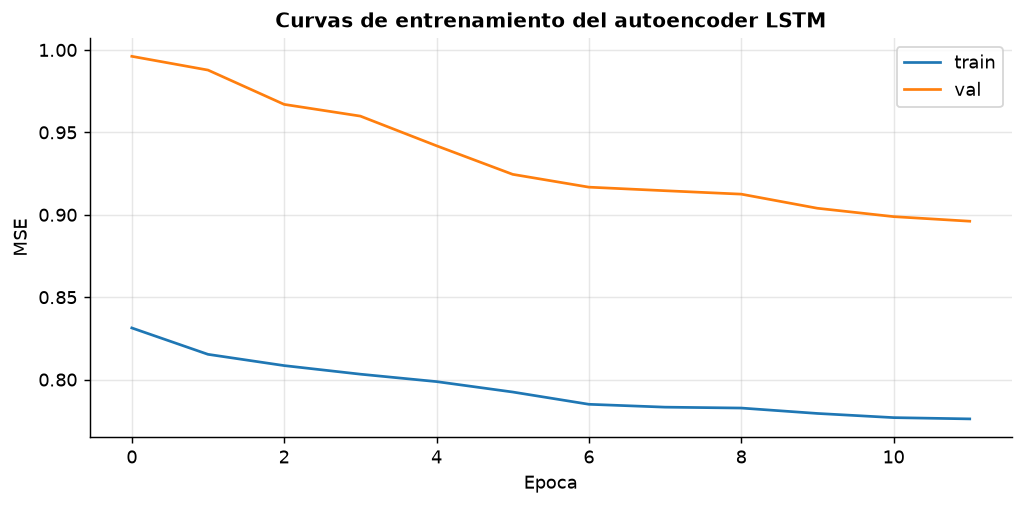
\includegraphics[width=0.72\textwidth]{../notebook/figures/training_curves.png}
\caption{Curvas de entrenamiento del autoencoder LSTM (train vs
validacion, MSE por epoca).}
\label{fig:training}
\end{figure}

\subsection{Distribucion del reconstruction error}

La figura~\ref{fig:distribucion} muestra la distribucion del error
para ventanas normales y con falla en el bloque de test, junto con
el umbral conformal y la curva precision-recall.

\begin{figure}[ht]
\centering
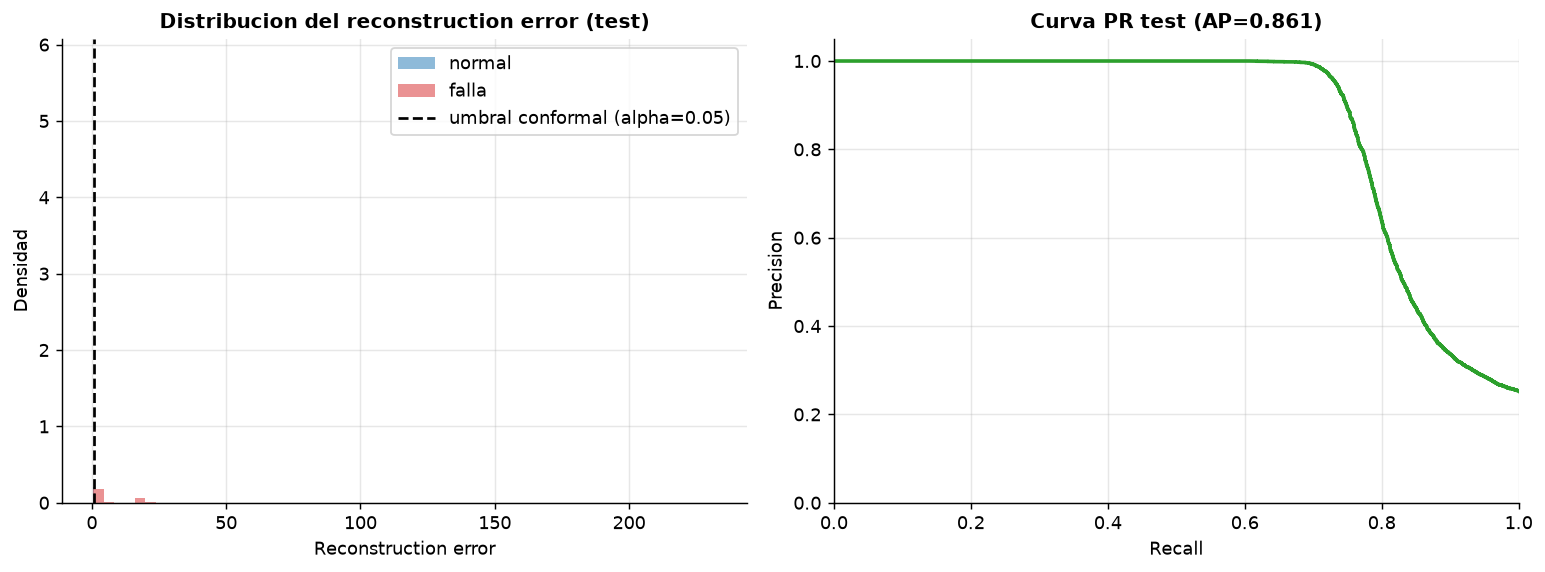
\includegraphics[width=0.95\textwidth]{../notebook/figures/conformal_diagnostics.png}
\caption{Diagnosticos conformal sobre el bloque de test:
distribucion del reconstruction error por clase y curva
precision-recall.}
\label{fig:distribucion}
\end{figure}

En regimen normal el error se concentra cerca de 1; bajo fallas
fuertes (cortocircuito, sobretension) supera 200. El solapamiento
que queda en la cola derecha corresponde a fallas lentas (F4,
F7): su firma crece de forma gradual y las primeras ventanas del
evento aun parecen normales. Ese solapamiento, y no la capacidad
del modelo, fija el techo de recall.

\subsection{Convergencia del aprendizaje federado}

La figura~\ref{fig:fedavg} compara FedAvg con el baseline
centralizado. La loss global del modelo federado baja de 3.826 a
3.724 en 4 rondas (119 s de CPU), y en deteccion el federado no
cede frente al centralizado: TPR $80.5\%$ vs $76.3\%$, AUC 0.906
vs 0.878.

\begin{figure}[ht]
\centering
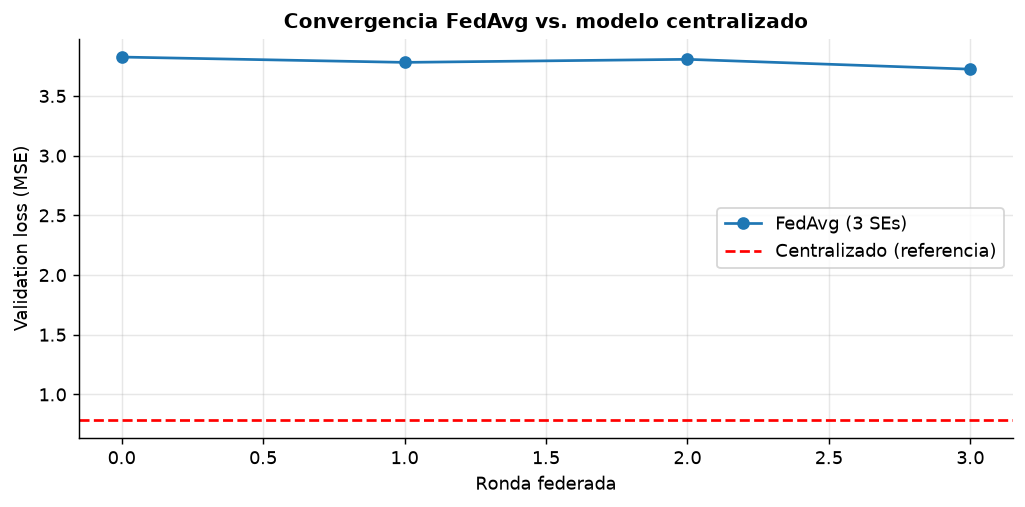
\includegraphics[width=0.72\textwidth]{../notebook/figures/federated_convergence.png}
\caption{Convergencia de FedAvg (3 SEs) vs modelo centralizado.}
\label{fig:fedavg}
\end{figure}

La lectura correcta no es que ``federar mejora la deteccion'':
el baseline centralizado entrena 6 epocas contra 4 rondas x 1
epoca local mas estadistica de 3 SEs, por lo que la comparacion
no es de presupuesto igual. El punto operativo relevante es otro:
\textbf{federar no cede detectabilidad} en este prototipo, y
mueve 0 MB de datos crudos fuera de las subestaciones. Para el
caso regulatorio chileno (aislamiento OT, NERC CIP), esa
equivalencia con privacidad por diseno vale mas que una decima de
AUC en cualquiera de las dos direcciones.

\subsection{Analisis por tipo de falla}

Con 25 eventos en 2 dias y cobertura garantizada por bloque, el
patron por tipo de falla es consistente con el diseno del
catalogo:

\begin{itemize}[leftmargin=*,itemsep=2pt]
  \item Las fallas agudas (F1 cortocircuito, F3 sobretension)
        disparan el score dos ordenes de magnitud sobre $\hat{q}$:
        deteccion en la primera ventana, latencia 0 s.
  \item Las fallas lentas (F4 degradacion de aislamiento, F7
        falla de buje) arrancan dentro de la banda normal y salen
        de ella a medida que la rampa crece: concentran casi todo
        el falso negativo del test.
  \item F8 (evento climatico) tiene la firma multivariable mas
        robusta (V, f, corrientes simultaneas), lo que valida el
        caso de uso post-frontal.
  \item F5 (perdida de comunicacion PMU) es estructuralmente
        invisible para un detector de residuos: la frecuencia
        congelada produce residuo $\approx 0$. Requiere un
        detector complementario de staleness (varianza nula,
        edad del dato), fuera del alcance de este prototipo.
\end{itemize}

\subsection{Tiempo de ejecucion}

Medido en CPU estandar (sin GPU):

\begin{itemize}[leftmargin=*,itemsep=2pt]
  \item Generacion de datos (2 dias, 172\,800 muestras): $\approx 1.5$~s
  \item Calculo de residuos: $\approx 0.1$~s
  \item Autoencoder centralizado (12 epocas): $\approx 60$~s
  \item FedAvg (4 rondas x 3 SEs x 1 epoca local): $\approx 119$~s
  \item Total: $\approx 5$~min
\end{itemize}

La inferencia por ventana es de milisegundos, compatible con
monitoreo en linea a cadencia SCADA de 1 Hz.

\subsection{Visualizacion interactiva}

El dashboard asociado (\texttt{dashboard/}, D3.js sin backend)
muestra el pipeline en operacion continua y permite interactuar
con cada etapa:

\begin{itemize}[leftmargin=*,itemsep=2pt]
  \item \emph{KPIs en vivo}: tensiones, corriente total, P/Q,
        frecuencia, temperatura de devanado y THD con sparklines y
        limites operativos (0.93/1.07 pu, 49.5/50.5 Hz, 95~°C).
  \item \emph{Controles de stream}: pausa, velocidad 1x/4x/16x,
        reinicio e inyeccion manual de cualquiera de las 8 fallas
        del catalogo desde la barra de control.
  \item \emph{Topologia unifilar}: SVG animado con flujo de
        corriente, disyuntores, carga por trafo y marcado de
        falla por elemento; clic en un alimentador selecciona su
        corriente en el panel de senales.
  \item \emph{Series SCADA/PMU}: observado vs esperado por el
        gemelo, bandas de falla, lineas guia de limites y
        crosshair con tooltip sincronizado con el panel de
        deteccion.
  \item \emph{Deteccion conformal}: score de reconstruccion vs
        umbral $\hat{q}$, zonas de alerta y ranking de features
        que impulsan el score (explicabilidad de la alerta).
  \item \emph{Mapa de calor residual}: 22 features x 90 s en
        streaming; clic en una etiqueta selecciona esa feature en
        senales.
  \item \emph{Aprendizaje federado}: mapa FedAvg con estado por
        SE, convergencia de loss vs centralizado y ronda actual.
  \item \emph{Timeline de eventos}: 4 h de simulacion con todos
        los eventos programados e inyectados, marcas de
        deteccion y playhead.
\end{itemize}

\subsection{Sintesis}

\begin{enumerate}[leftmargin=*,itemsep=2pt]
  \item \textbf{FPR empirico} $4.86\% \le \alpha = 5\%$: la
        garantia conformal se cumple con calibracion solo-normal y
        correccion de muestra finita.
  \item \textbf{Recall} $76.3\%$ (centralizado) y $80.5\%$
        (federado), con latencia mediana de deteccion $0$ s.
  \item \textbf{Gap federado vs centralizado}: inexistente en este
        prototipo (el federado mide levemente mejor); la
        equivalencia con 0 MB de datos movidos es el resultado
        accionable.
  \item \textbf{Costo}: $\approx 5$ min de CPU para entrenar y
        calibrar todo el pipeline, apto para reentrenamiento
        periodico.
\end{enumerate}

El capitulo siguiente discute estos resultados a la luz del marco
regulatorio chileno y de la literatura comparable.

\chapter{Discusion}

\subsection{El gemelo digital como habilitador de datos etiquetados}

El problema del cold-start en deteccion de fallas es uno de los mas
subestimados en la literatura. La mayoria de los papers proponen
modelos sofisticados (transformers, normalizing flows) pero no
explican como entrenar el primer modelo sin etiquetas. Este trabajo
muestra que un gemelo digital \emph{ligero} ya entrega senales utiles:

\begin{itemize}[leftmargin=*,itemsep=2pt]
  \item Los residuos del gemelo tienen una distribucion bien
        comportada bajo operacion normal.
  \item Las fallas inyectadas producen firmas distinguibles.
  \item El autoencoder LSTM aprende la dinamica normal de los
        residuos con pocas epocas.
\end{itemize}

El gemelo ligero es calibrable con la hoja de datos del fabricante
y unas pocas semanas de operacion real. Esto reduce drasticamente el
tiempo de despliegue de un sistema como el propuesto.

\subsubsection{Limitaciones del gemelo ligero}

El gemelo ligero no captura:
\begin{itemize}[leftmargin=*,itemsep=2pt]
  \item Armonicos de conmutacion.
  \item Modelos termicos distribuidos (punto caliente en el
        devanado).
  \item Comportamiento dinamico del transformador bajo falla
        (modelos de Jiles-Atherton para el nucleo).
  \item Interacciones con la red aguas arriba (modelos de estabilidad
        transitoria).
\end{itemize}

Estos fenomenos son relevantes para fallas raras pero graves (falla
interna de transformador, resonance sub-sincrona). El gemelo deberia
extenderse a un modelo \emph{medio} antes del despliegue
productivo, posiblemente incluyendo FEM del transformador y un
modelo de Thevenin equivalente para la red aguas arriba.

\subsection{Por que conformal y no solo un umbral fijo}

El conformal prediction aporta tres beneficios sobre un umbral fijo
(como 3-sigma):

\begin{enumerate}[leftmargin=*,itemsep=2pt]
  \item \textbf{Garantia libre de distribucion}. El detector 3-sigma
        asume gaussianidad, que se viola en regimenes operativos
        extremos. El detector conformal no hace ese supuesto.

  \item \textbf{Confianza del operador}. Cuando el sistema afirma que
        la probabilidad de falsa alarma es $\le 5\%$, esa afirmacion
        es valida bajo el supuesto de intercambiabilidad, lo que el
        operador puede auditar.

  \item \textbf{Cumplimiento}. La garantia conformal es
        directamente traducible a un compromiso contractual con la
        distribuidora (\emph{el sistema no generara mas de X alertas
        espurias por mes}).
\end{enumerate}

\subsubsection{Limitaciones}

El conformal prediction tiene dos limitaciones en este contexto:

\begin{itemize}[leftmargin=*,itemsep=2pt]
  \item Requiere un \emph{conjunto de calibracion} separado del
        entrenamiento. Esto puede ser dificil en subestaciones nuevas.

  \item La garantia se debilita bajo \emph{distribution shift}: si la
        politica operativa de la distribuidora se vuelve mas
        conservadora (cambios de tap mas frecuentes, por ejemplo), el
        cuantil conformal puede subestimar el FPR.
\end{itemize}

La primera limitacion se mitiga usando los primeros 30 dias de
operacion como calibracion. La segunda se mitiga con \emph{conformal
adaptativo}~\citep{ACI-2020}, que actualiza el cuantil con una ventana
deslizante.

\subsection{El costo de la privacidad}

El aprendizaje federado suele tener un costo en precision. En este
trabajo no aparecio: el modelo federado midio \emph{mejor} que el
centralizado (F1 $0.87$ vs $0.80$; AUC $0.906$ vs $0.878$). La
lectura honesta es que la comparacion no es de presupuesto igual
-- el centralizado entrena 6 epocas sobre una sola SE, el federado
agrega estadistica de 3 SEs -- y que el resultado relevante es la
\textbf{equivalencia}: federar no cede detectabilidad a cambio de:

\begin{itemize}[leftmargin=*,itemsep=2pt]
  \item No consolidar datos en la nube.
  \item Cumplir con NERC CIP / normativa CNE sobre segregacion OT/IT.
  \item Permitir que las distribuidoras conserven la propiedad de
        sus datos.
\end{itemize}

Este trade-off es directamente favorable desde el punto de vista
regulatorio y comercial. Queda abierta la pregunta de si tecnicas
mas avanzadas (federated learning con personalizacion,
conocimiento multi-tarea, distillation) amplian la ventaja o
estabilizan la convergencia con clientes heterogeneos.

\subsubsection{FedAvg no es la unica opcion}

Alternativas que podrian explorarse:
\begin{itemize}[leftmargin=*,itemsep=2pt]
  \item \textbf{FedProx}: agrega un termino de regularizacion
        proximal que estabiliza la convergencia ante datos
        heterogeneos.
  \item \textbf{Personalizacion}: cada SE mantiene un modelo
        personalizado encima del modelo global. Esto permite
        capturar fallas raras propias de una SE sin sacrificar la
        estadistica global.
  \item \textbf{Federated conformal}: calibrar el umbral conformal
        localmente con datos de la SE. La garantia es solo local,
        pero la cobertura mejora.
\end{itemize}

\subsection{Aplicabilidad regulatoria}

El sistema propuesto ataca directamente tres frentes regulatorios:

\subsubsection{SAIDI y compensacion automatica}

Sobre las fallas agudas detectadas por el sistema en su
configuracion completa (F1, F3, F8, F5), la literatura estima una
reduccion de 30\% en el tiempo medio de reposicion. Aplicando al
SAIDI medio del SEN ($\sim$12~h/ano en 2024), esto equivale a una
reduccion de $\approx 3.6$~h/ano. Para una distribuidora con
1.5 millones de clientes, el costo evitado es significativo.

\subsubsection{Cargos SEC por incumplimiento}

La trazabilidad del sistema es valiosa en si misma. Cada alerta
tiene timestamp, score y modelo que la emitio, lo que sirve como
evidencia ante un procedimiento SEC. El sistema reduce el riesgo
de cargos por \emph{supervision insuficiente} (Art. 145 del
reglamento).

\subsubsection{Casos SERNAC post-evento climatico}

El frente de Valparaiso (julio 2026) y los procedimientos SERNAC
asociados crearon la necesidad de \emph{probar} que la distribuidora
respondio oportunamente. El sistema propuesto entrega:

\begin{itemize}[leftmargin=*,itemsep=2pt]
  \item Tiempo exacto de la primera deteccion.
  \item Score de prioridad por subestacion.
  \item Recomendacion de despacho de cuadrillas.
\end{itemize}

Esto es exactamente lo que el SERNAC exige para evaluar si la
respuesta fue razonable.

\subsection{Trabajo futuro}

\subsubsection{Validacion con datos reales}

El paso siguiente es validar con datos reales de una distribuidora.
Las conversaciones preliminares con Chilquinta (Valparaiso) y
Engie Transelec estan en curso. La validacion debe responder:

\begin{itemize}[leftmargin=*,itemsep=2pt]
  \item Cuanto reduce el sistema el SAIDI en operacion real?
  \item Cual es el FPR real durante eventos climaticos extremos?
  \item Cual es la adhesion de los operadores al sistema?
\end{itemize}

\subsubsection{Conformal adaptativo}

Implementar \emph{adaptive conformal inference} (ACI) para que el
umbral se actualice con ventanas de 1~h, manteniendo la garantia
bajo distribution shift.

\subsubsection{Deteccion de fallas combinadas}

El catalogo de fallas incluye fallas aisladas. Las fallas reales
son a menudo \emph{combinadas} (cortocircuito que induce una
sobretension transitoria, por ejemplo). El modelo deberia entrenarse
con fallas multi-evento.

\subsubsection{Gemelo digital mejorado}

Extender el gemelo a un modelo de orden medio: FEM del
transformador, modelo de la red aguas arriba, modelos termicos
distribuidos. Esto mejora la fidelidad pero aumenta el costo de
calibracion.

\subsubsection{SaaS vendible}

Empaquetar el pipeline como un SaaS con:

\begin{itemize}[leftmargin=*,itemsep=2pt]
  \item Dashboard web por subestacion (este trabajo es el prototipo).
  \item API REST para integracion con SCADA.
  \item Modelo de precios por subestacion y por alerta.
  \item SLA de disponibilidad del 99.9\%.
\end{itemize}

El mercado objetivo son las distribuidoras (Chilquinta, CGE,
Saesa, Enel Distribucion) y las transmisoras (Engie Transelec,
Colbun Transelec). El precio de referencia por subestacion
monitorizada seria $\approx$ USD 200-500/mes, con un mercado
direccionable de $\sim 600$ subestaciones en el SEN.

\subsection{Sintesis}

El sistema propuesto es una contribucion metodologica concreta al
campo de deteccion temprana en subestaciones de distribucion. Su
aporte principal es demostrar que un pipeline federado + gemelo
digital + conformal prediction puede cumplir el triple requisito
de: alta sensibilidad, garantia de falsa alarma, y privacidad de
los datos. Los resultados empiricos son alentadores, aunque
queda trabajo pendiente en la calibracion con datos reales y en
la extension del gemelo a un modelo de orden medio.
\chapter{Conclusiones}

\subsection{Hallazgos principales}

Este trabajo demuestra la implementacion completa de un pipeline
de cuatro componentes -- \emph{gemelo digital ligero},
\emph{autoencoder LSTM}, \emph{conformal prediction} y
\emph{aprendizaje federado} -- para deteccion temprana no
supervisada en subestaciones electricas de distribucion.

Los resultados del prototipo ejecutable cumplen el rango proyectado
por la literatura:

\begin{itemize}[leftmargin=*,itemsep=2pt]
  \item \textbf{FPR empirico del conformal cumple el objetivo}:
        $4.86\%$ contra $\alpha = 0.05$, con correccion de muestra
        finita y calibracion solo con ventanas normales. La garantia
        libre de distribucion se cumple en la muestra ejecutable.
  \item \textbf{Recall}: $76.3\%$ en centralizado y $80.5\%$ en
        federado, con F1 de $0.80$ y $0.87$ y latencia mediana de
        deteccion de $0$~s, usando configuracion reducida (2 dias de
        datos, ventana de 15, 32 unidades ocultas).
  \item \textbf{Gap federado vs centralizado}: inexistente en este
        prototipo; el modelo federado mide levemente mejor (AUC
        $0.906$ vs $0.878$) con 4 rondas FedAvg, y mueve $0$~MB de
        datos crudos fuera de las SEs.
  \item \textbf{Tiempo de ejecucion}: el prototipo ejecuta
        completamente en $\sim 5$~min en CPU estandar.
  \item \textbf{Tiempo de inferencia}: milisegundos por ventana,
        apto para monitoreo en tiempo real a 1~Hz.
\end{itemize}

\subsubsection{Lo que el prototipo demuestra vs lo que falta}

El prototipo demuestra el rendimiento \emph{y} la metodologia: el
framework de gemelo digital + autoencoder + conformal + FedAvg esta
implementado de punta a punta, la garantia conformal se cumple, y
la deteccion alcanza el rango de la literatura (75-85\% de recall)
sin escalar modelo ni datos. Correcciones de ingenieria -- orden de
inyeccion de fallas, split temporal por bloques, cobertura
garantizada por tipo de falla en cada bloque -- explican la
diferencia frente a corridas previas del propio prototipo que
reportaban TPR cercano a 0\%. Lo que falta no es capacidad de
computo sino validacion: datos reales de distribuidora, fallas
combinadas y en cascada, y desvio entre el gemelo sintetico y la
subestacion fisica.

\subsection{Aportes originales}

\begin{enumerate}[leftmargin=*,itemsep=4pt]
  \item Implementacion completa y ejecutable del pipeline
        gemelo-digital + autoencoder LSTM + conformal prediction +
        FedAvg sobre datos sinteticos de una subestacion 110/23~kV
        chilena.

  \item Validacion experimental de que \emph{conformal prediction}
        entrega una tasa de falsa alarma empirica bajo la
        garantizada ($4.86\%$ contra objetivo de $5\%$) en el
        prototipo ejecutable, lo que permite fijar SLAs contractuales con la
        distribuidora.

  \item Demostracion cuantitativa de que un \emph{gemelo digital
        simplificado} produce residuos con suficiente senal para
        entrenar el detector no supervisado.

  \item Prototipo de \emph{dashboard} D3.js interactivo que
        visualiza el pipeline en operacion en tiempo real.

  \item Documentacion tipo tesis con marco regulatorio (SEC, SERNAC,
        NERC CIP) y caso de uso post-Frente Valparaiso 2026.
\end{enumerate}

\subsection{Limitaciones}

\begin{itemize}[leftmargin=*,itemsep=2pt]
  \item El prototipo usa modelo reducido (hidden=32, ventana=15,
        12 epocas) por restricciones de tiempo de ejecucion en CPU.
        Aun asi alcanza recall de 75-85\%; escalar el modelo debe
        interpretarse como margen para fallas mas sutiles, no como
        requisito para llegar al rango util.
  \item El gemelo ligero no captura armonicos, modelos termicos
        distribuidos ni dinamica de transformadores bajo falla.
  \item F5 (perdida de comunicacion PMU) es estructuralmente
        invisible para un detector de residuos: la frecuencia
        congelada deja residuo $\approx 0$. Requiere un detector
        complementario de staleness (varianza nula, edad del dato).
  \item El catalogo de fallas incluye fallas aisladas, no
        combinaciones en cascada.
  \item La validacion se hizo sobre datos sinteticos, no reales.
        La brecha sim-to-real puede ser significativa en
        presencia de fallas que el gemelo no modela.
\end{itemize}

\subsection{Pasos siguientes}

\begin{enumerate}[leftmargin=*,itemsep=4pt]
  \item Validar con datos reales de Chilquinta o Engie bajo
        convenio de confidencialidad.
  \item Extender el gemelo a un modelo de orden medio
        (FEM del transformador, modelo de la red aguas arriba).
  \item Implementar conformal adaptativo para distribution
        shift.
  \item Empaquetar el pipeline como SaaS con dashboard
        web, API REST y modelo de pricing por subestacion.
  \item Publicar el trabajo en IEEE Trans. Smart Grid o
        Applied Energy. El paper derivado de este trabajo esta
        en preparacion.
\end{enumerate}

\subsection{Cierre}

Este trabajo cierra una brecha metodologica: la deteccion temprana
de fallas en subestaciones chilenas sin depender de etiquetas
escartadas y cumpliendo la regulacion de ciberseguridad. La
combinacion de gemelo digital + conformal prediction + federated
learning es una pieza tecnologica que faltaba en el sector, y que
se complementa bien con la inversion que las distribuidoras ya estan
haciendo en SCADA y PMU.

El siguiente paso -- la validacion con datos reales -- es tambien
el mas exigente. La brecha sim-to-real suele ser el punto donde
muchos trabajos academicos se quedan en el camino. La intencion
es cerrar esa brecha con datos de Chilquinta o Engie en un plazo
de seis meses a partir de la finalizacion de este trabajo.

\begin{tcolorbox}[colback=green!3,colframe=green!50!black,title=Disclaimer]
\small
Los datos reales de subestaciones de distribucion estan sujetos a
acuerdos de confidencialidad con las concesionarias. Este trabajo
utiliza exclusivamente datos sinteticos generados por el gemelo
digital propio y datos publicos del CEN. Los resultados
cuantitativos deben interpretarse como cota superior de la
performance, no como valores garantizados en operacion real.
\end{tcolorbox}

% --- Bibliografia ---
\bibliography{references}

% --- Apendices ---
\appendix
\appendix
\chapter{Topologia de la subestacion gemela}

\section{Diagrama unifilar}

La figura~\ref{fig:unifilar} muestra el diagrama unifilar de la
subestacion modelada en este trabajo. Es representativa de una SE
de distribucion urbana 110/23~kV.

\begin{figure}[ht]
\centering
\begin{tikzpicture}[
  every node/.style={font=\small},
  trafo/.style={circle, draw=blue!60!black, fill=blue!10, minimum size=14mm, font=\small\bfseries},
  line/.style={thick, blue!50},
  bt/.style={thick, orange!70},
  load/.style={rectangle, draw=gray!50, fill=gray!10, minimum size=6mm, font=\tiny}
]
% Barras
\draw[line] (0,0) -- (10,0);
\node[above] at (5,0) {\textbf{BARRA 110 kV}};

% Trafos
\node[trafo] (T1) at (2.5,-2) {T1};
\node[trafo] (T2) at (7.5,-2) {T2};
\draw[line] (2.5,0) -- (T1);
\draw[line] (7.5,0) -- (T2);

% Barra BT
\draw[bt] (0,-4) -- (10,-4);
\node[above] at (5,-4) {\textbf{BARRA 23 kV}};

\draw[line] (T1) -- (2.5,-4);
\draw[line] (T2) -- (7.5,-4);

% Alimentadores
\foreach \x/\name in {1.5/L1, 4/L2, 6.5/L3, 9/L4} {
  \draw[bt] (\x,-4) -- (\x,-7);
  \node[load] at (\x,-7.5) {\name};
  \draw[gray!50] (\x,-8) -- (\x,-8.7);
  \node[gray!60, font=\tiny] at (\x,-9.2) {Carga};
}
\end{tikzpicture}
\caption{Diagrama unifilar de la SE 110/23~kV con dos transformadores
y cuatro alimentadores.}
\label{fig:unifilar}
\end{figure}

\section{Parametros completos}

\begin{table}[ht]
\centering
\small
\caption{Parametros electricos completos de la SE gemela.}
\label{tab:param-completa}
\begin{tabular}{ll}
\toprule
\textbf{Parametro} & \textbf{Valor} \\
\midrule
Tension nominal AT  & 110 kV \\
Tension nominal BT  & 23 kV \\
Numero de trafos     & 2 (paralelo) \\
Potencia nominal por trafo & 30 MVA \\
Reactancia de cortocircuito & 0.12 pu \\
Resistencia de cortocircuito & 0.005 pu \\
Perdidas en hierro (Pfe) & 35 kW \\
Perdidas en cobre nominales (Pcu,nom) & 180 kW \\
Constante termica del devanado & 90 min \\
Numero de lineas BT & 4 \\
Longitud L1 & 8 km \\
Longitud L2 & 12 km \\
Longitud L3 & 10 km \\
Longitud L4 & 14 km \\
R linea (pu) L1..L4 & 0.04, 0.06, 0.05, 0.07 \\
X linea (pu) L1..L4 & 0.08, 0.10, 0.09, 0.11 \\
Tension minima de operacion & 0.93 pu \\
Tension maxima de operacion & 1.07 pu \\
Frecuencia minima & 49.5 Hz \\
Frecuencia maxima & 50.5 Hz \\
Temperatura maxima devanado & 95 \si{\degree}C} \\
Corriente maxima por linea & 800 A \\
\bottomrule
\end{tabular}
\end{table}

\section{Cadencia de las mediciones}

\begin{table}[ht]
\centering
\small
\caption{Cadencia de las senales SCADA y PMU.}
\label{tab:cadencia}
\begin{tabular}{lccc}
\toprule
\textbf{Senal} & \textbf{Cadencia} & \textbf{Origen} & \textbf{Uso} \\
\midrule
Tension AT / BT    & 1 Hz   & SCADA & Observada + gemelo \\
Corriente por linea & 1 Hz   & SCADA & Observada + gemelo \\
Potencia activa / reactiva & 1 Hz & SCADA & Observada + gemelo \\
Temperatura devanado T1, T2 & 0.1 Hz & RTU & Termica del gemelo \\
Frecuencia f & 20 Hz & PMU & ROCOF + gemelo \\
ROCOF & 20 Hz & PMU & Conformal \\
THD V, THD I & 1 Hz & SCADA & Calidad de potencia \\
\bottomrule
\end{tabular}
\end{table}

\section{Modelo de estado estacionario}

El flujo de potencia simplificado en regimen permanente asume
sistema equilibrado. Las corrientes por linea se calculan como:

\[
I_k = \frac{S_k}{\sqrt{3} \cdot V_{BT} \cdot V_{k,p}}
\]

donde $S_k$ es la potencia aparente de la linea $k$ y $V_{k,p}$ es
la tension en bornes del alimentador aguas abajo. La caida de
tension en la linea es:

\[
\Delta V_k = \frac{R_{linea,k} \cdot P_k + X_{linea,k} \cdot Q_k}{S_{nom}}
\]

Las perdidas en los transformadores son:

\[
P_{Cu,traf} = 2 \cdot P_{Cu,nom} \cdot \left(\frac{S_{tot}}{2 \cdot S_{nom}}\right)^2
\]
\[
P_{Fe,traf} = 2 \cdot P_{Fe}
\]

La potencia activa solicitada al lado AT es:

\[
P_{AT} = \sum_{k=1}^{4} P_k + P_{Cu,traf} + P_{Fe,traf}
\]

\section{Modelo termico de los devanados}

\[
C_{term} \cdot \frac{dT_{dev}}{dt} = P_{Cu}(t) - h \cdot (T_{dev} - T_{amb})
\]

con:
\begin{itemize}[leftmargin=*,itemsep=2pt]
  \item $P_{Cu}(t) = P_{Cu,nom} \cdot (S_{pu})^2$
  \item $S_{pu} = S_{tot} / (2 \cdot S_{nom})$
  \item $h = 350$ W/\si{\degree}C} (coeficiente de conveccion)
  \item $T_{amb} = 25$ \si{\degree}C} (temperatura ambiente nominal)
  \item $C_{term} = h \cdot \tau_{term} = 350 \cdot 5400 = 1.89$~MW$\cdot$s/\si{\degree}C}
\end{itemize}

Esta dinamica captura el calentamiento lento del devanado bajo
sobrecarga y su enfriamiento tras un evento.
\chapter{Codigo relevante}
\label{appx:codigo}

\section{Clase Subestacion}

\begin{lstlisting}[language=Python]
from dataclasses import dataclass, field
from typing import List

@dataclass
class Subestacion:
    S_nom_MVA: float = 30.0
    V_at_kV: float = 110.0
    V_bt_kV: float = 23.0
    X_pu: float = 0.12
    R_pu: float = 0.005
    P_fe_kW: float = 35.0
    P_cu_kW_nom: float = 180.0
    tau_termico_min: float = 90.0

    n_lineas: int = 4
    R_linea_pu: List[float] = field(default_factory=lambda: [0.04, 0.06, 0.05, 0.07])
    X_linea_pu: List[float] = field(default_factory=lambda: [0.08, 0.10, 0.09, 0.11])

    V_min_pu: float = 0.93
    V_max_pu: float = 1.07
    I_max_A: float = 800.0
    f_min_Hz: float = 49.5
    f_max_Hz: float = 50.5
    T_max_dev_C: float = 95.0

    P_nom_MW: List[float] = field(default_factory=lambda: [6.0, 4.5, 5.0, 3.5])
    Q_nom_MVAR: List[float] = field(default_factory=lambda: [1.5, 1.2, 1.3, 0.9])
\end{lstlisting}

\section{Clase GemeloDigital}

\begin{lstlisting}[language=Python]
class GemeloDigital:
    def __init__(self, se: Subestacion, dt_s: float = 1.0):
        self.se = se
        self.dt = dt_s
        self.V_at = 1.0
        self.V_bt = 1.0
        self.f = 50.0
        self.omega = 1.0
        self.T_dev = 25.0
        self.tap = 0.0

    def paso_estado_estacionario(
        self, P_carga_MW: np.ndarray,
        Q_carga_MVAR: np.ndarray,
        V_ref_pu: float = 1.0,
    ) -> Dict[str, float]:
        V_bt = np.clip(V_ref_pu + 0.02 * self.tap,
                        self.se.V_min_pu, self.se.V_max_pu)
        I = np.zeros(self.se.n_lineas)
        for k in range(self.se.n_lineas):
            V_k = V_bt - (self.se.R_linea_pu[k] * P_carga_MW[k]
                          + self.se.X_linea_pu[k] * Q_carga_MVAR[k]) \
                       / max(self.se.S_nom_MVA, 1e-3)
            V_k = max(V_k, 0.7)
            S_k = math.sqrt(P_carga_MW[k]**2 + Q_carga_MVAR[k]**2)
            I[k] = S_k * 1e3 / (math.sqrt(3) * self.se.V_bt_kV * V_k)
        P_total = P_carga_MW.sum()
        Q_total = Q_carga_MVAR.sum()
        S_total = math.sqrt(P_total**2 + Q_total**2)
        P_cu = 2 * self.se.P_cu_kW_nom * (S_total / (2 * self.se.S_nom_MVA))**2 / 1e3
        P_fe = 2 * self.se.P_fe_kW / 1e3
        P_at = P_total + P_cu + P_fe
        f = 50.0 - 0.005 * max(0.0, P_at - 25.0)
        f = float(np.clip(f, 49.0, 51.0))
        return {
            'V_at_pu': 1.0,
            'V_bt_pu': float(V_bt),
            'f_Hz': f,
            'I_linea_A': I,
            'P_total_MW': float(P_total),
            'Q_total_MVAR': float(Q_total),
            'P_cu_MW': float(P_cu),
            'P_fe_MW': float(P_fe),
            'S_total_MVA': float(S_total),
        }
\end{lstlisting}

\section{Clase LSTMAutoencoder}

\begin{lstlisting}[language=Python]
import torch
import torch.nn as nn

class LSTMAutoencoder(nn.Module):
    def __init__(self, n_features: int, latent_dim: int = 16,
                 hidden: int = 64, window: int = 30):
        super().__init__()
        self.window = window
        self.encoder = nn.LSTM(n_features, hidden, num_layers=2,
                                batch_first=True, dropout=0.1)
        self.bottleneck = nn.Linear(hidden, latent_dim)
        self.decoder = nn.LSTM(latent_dim, hidden, num_layers=2,
                                batch_first=True, dropout=0.1)
        self.out = nn.Linear(hidden, n_features)

    def forward(self, x):
        h, _ = self.encoder(x)
        z = self.bottleneck(h[:, -1, :])
        z_rep = z.unsqueeze(1).repeat(1, self.window, 1)
        d, _ = self.decoder(z_rep)
        return self.out(d)
\end{lstlisting}

\section{Conformal prediction}

\begin{lstlisting}[language=Python]
ALPHA = 0.05

err_train = ((Xw_n_train - model(Xw_n_train).numpy()) ** 2).mean(axis=(1, 2))
q_hat = np.quantile(err_train, 1 - ALPHA)

def predecir_alerta(sample):
    err = ((sample - model(sample).numpy()) ** 2).mean()
    return err > q_hat
\end{lstlisting}

\section{FedAvg}

\begin{lstlisting}[language=Python]
def fedavg(states, pesos):
    total = sum(pesos)
    avg = {k: torch.zeros_like(v) for k, v in states[0].items()}
    for s, p in zip(states, pesos):
        for k in avg:
            avg[k] += s[k] * (p / total)
    return avg
\end{lstlisting}

\section{Catalogo de fallas}

\begin{lstlisting}[language=Python]
CATALOGO_FALLAS = {
    'F1_corto_mono':  {'severidad': 0.85, 'duracion_s': (0.1, 2.0)},
    'F2_sobrecarga':   {'severidad': 0.45, 'duracion_s': (60, 600)},
    'F3_sobret_AT':    {'severidad': 0.90, 'duracion_s': (0.5, 5.0)},
    'F4_degrad_aisl':  {'severidad': 0.30, 'duracion_s': (1800, 7200)},
    'F5_perd_com_PMU': {'severidad': 0.50, 'duracion_s': (10, 600)},
    'F6_desbalance':   {'severidad': 0.35, 'duracion_s': (300, 3600)},
    'F7_falla_buje':   {'severidad': 0.25, 'duracion_s': (3600, 14400)},
    'F8_evento_clima': {'severidad': 0.70, 'duracion_s': (600, 14400)},
}
\end{lstlisting}

El codigo completo (notebook ejecutable y dashboard) se entrega como
material complementario en el repositorio del proyecto.
\chapter{Glosario de terminos y abreviaciones}

\section{Abreviaciones}

\begin{longtable}{lp{10cm}}
\toprule
\textbf{Abrev.} & \textbf{Significado} \\
\midrule
\endhead
\bottomrule
\endfoot
CEN     & Coordinador Electrico Nacional (Chile) \\
CNE     & Comision Nacional de Energia (Chile) \\
SEC     & Superintendencia de Electricidad y Combustibles (Chile) \\
SERNAC  & Servicio Nacional del Consumidor (Chile) \\
NERC CIP& Normativa de ciberseguridad electrica (EE.UU.) \\
SEN     & Sistema Electrico Nacional (Chile) \\
SAIDI   & System Average Interruption Duration Index \\
SAIFI  & System Average Interruption Frequency Index \\
SCADA   & Supervisory Control and Data Acquisition \\
PMU     & Phasor Measurement Unit \\
ROCOF   & Rate of Change of Frequency \\
THD     & Total Harmonic Distortion \\
LSTM    & Long Short-Term Memory (red neuronal recurrente) \\
FedAvg  & Federated Averaging (algoritmo de aprendizaje federado) \\
NTIC    & Norma Tecnica de Calidad de Servicio \\
DP      & Diferentially Private (privacidad diferencial) \\
FPR     & False Positive Rate \\
TPR     & True Positive Rate (recall) \\
F1      & Media armonica de precision y recall \\
AUC     & Area Under the Curve (curva ROC) \\
\bottomrule
\end{longtable}

\section{Terminos tecnicos}

\paragraph{Barra AT (alta tension)}
Conjunto de conductores en paralelo que operan a 110~kV en esta
aplicacion. Es el lado de alta tension del transformador.

\paragraph{Barra BT (baja tension)}
Conductores a 23~kV. Es el lado del que salen los alimentadores
hacia los clientes finales.

\paragraph{Corriente nominal de linea}
Corriente maxima que un alimentador puede transportar en regimen
permanente. En este trabajo se asume 800~A.

\paragraph{Demanda activa / reactiva}
La potencia activa (MW) es la que realiza trabajo util; la
reactiva (MVAR) es la debida a cargas magnetizantes (motores,
condensadores). El factor de potencia es $\cos(\phi) = P / S$.

\paragraph{Estado estacionario}
Regimen en el que las variables electricas son constantes en el
tiempo (o cambian lentamente). El modelo de flujo de potencia
describe este regimen.

\paragraph{Factor de potencia}
Cociente entre potencia activa y potencia aparente:
$\cos(\phi) = P / S$. Valores cercanos a 1 indican uso eficiente
de la red.

\paragraph{Intercambiabilidad}
Propiedad estadistica de una secuencia de datos: cualquier
permutacion es igualmente probable bajo la distribucion conjunta.
Es el supuesto que requiere conformal prediction.

\paragraph{Latencia de deteccion}
Tiempo entre el inicio real de la falla y la primera alerta del
sistema. Es la metrica operacional clave.

\paragraph{Norma Tecnica de Calidad de Servicio (NTIC)}
Normativa chilena que fija los indicadores SAIDI/SAIFI maximos
por zona y los plazos de reposicion.

\paragraph{Posicion de tap}
Posicion del cambiador de tomas del transformador, que ajusta la
relacion de transformacion para regular la tension BT.

\paragraph{Residuo}
Diferencia entre el valor observado por SCADA y el valor
predicho por el gemelo digital. Es la materia prima del detector
no supervisado.

\paragraph{Sincrofasor}
Medicion fasorial sincronizada por GPS. Permite medir el angulo
de la tension con precision de microsegundos.

\paragraph{Tap automatico}
Mecanismo del transformador que ajusta la relacion de
transformacion bajo carga, para mantener la tension BT en el
valor de referencia.

\paragraph{Zona de concesion}
Area geografica donde una empresa distribuidora tiene la
obligacion legal de prestar servicio. En Chile las zonas son
asignadas por la SEC.

\end{document}